\documentclass[aps,prl,reprint]{revtex4-1}
\usepackage{blindtext}

\usepackage{amsmath}
\usepackage{graphicx}
\usepackage{commath}
\usepackage{siunitx}
\usepackage{tabularx}
\usepackage{subcaption}

\usepackage{float}

\usepackage{graphicx}


\usepackage[b]{esvect}

\newcommand{\de}{\mathrm{d}}
\newcommand{\vcc}{V_\text{cc}}

\graphicspath{ {images/} }
\begin{document}
\title{Unit 3: Diode circuits and DC Power}
\author{Xueqi Li}
% \email{xueqi.li@stonybrook.edu}
\thanks{Partner: Tianming Hai}
% \author{partner Tianming Hai}
\noaffiliation
\date{Feb 23, 2018}


% \begin{abstract}
% Here I tell what I have done... And I have done a lot but it is hard to tell what exactly I have done...
% \end{abstract}

\maketitle

\section{Introduction}  
    \subsection{Semiconductor}
    Simiconductor is usually made by doping silicon with impurities so that to form n-type semiconductor, which have carriers as electrons, and p-type semiconductor, which have carriers as carriers as hole.
    \subsection{p–n Junction}
    In the interface between two tpyes of semiconductor, a p-n junction is formed. In such interface, the carriers of two type of semiconductor are attract and form a electric field in the interface, which prevent more carriers been attract. When an external electric field been apply, if the external electric field is in the same direction of the interface electric field, it strengthen the interface electric field so that no charge can flow through the interface. On the other hand, if the external electric field is the opposite direction of interface electric field, it weak the interface electric field so that charge can flow freely along the electric field. However, in such casem a voltage drop of around 0.65V is happened in the p-n junction.
    \subsection{Diode}
    A diode can be form by a p-n junction with two types of semiconductor. The principle of a diode is the p-n junction. Thus, when voltage is larger than 0.65V, the diode is same as wire (with 0.65V voltage drop), and when voltage is smaller than 0.65V, it is a open circuit. In a very low voltage, it will allow charge to flow again, which is not discussed here.
    \subsection{Clipping Circuit}
    \begin{figure}[h]
        \centering
        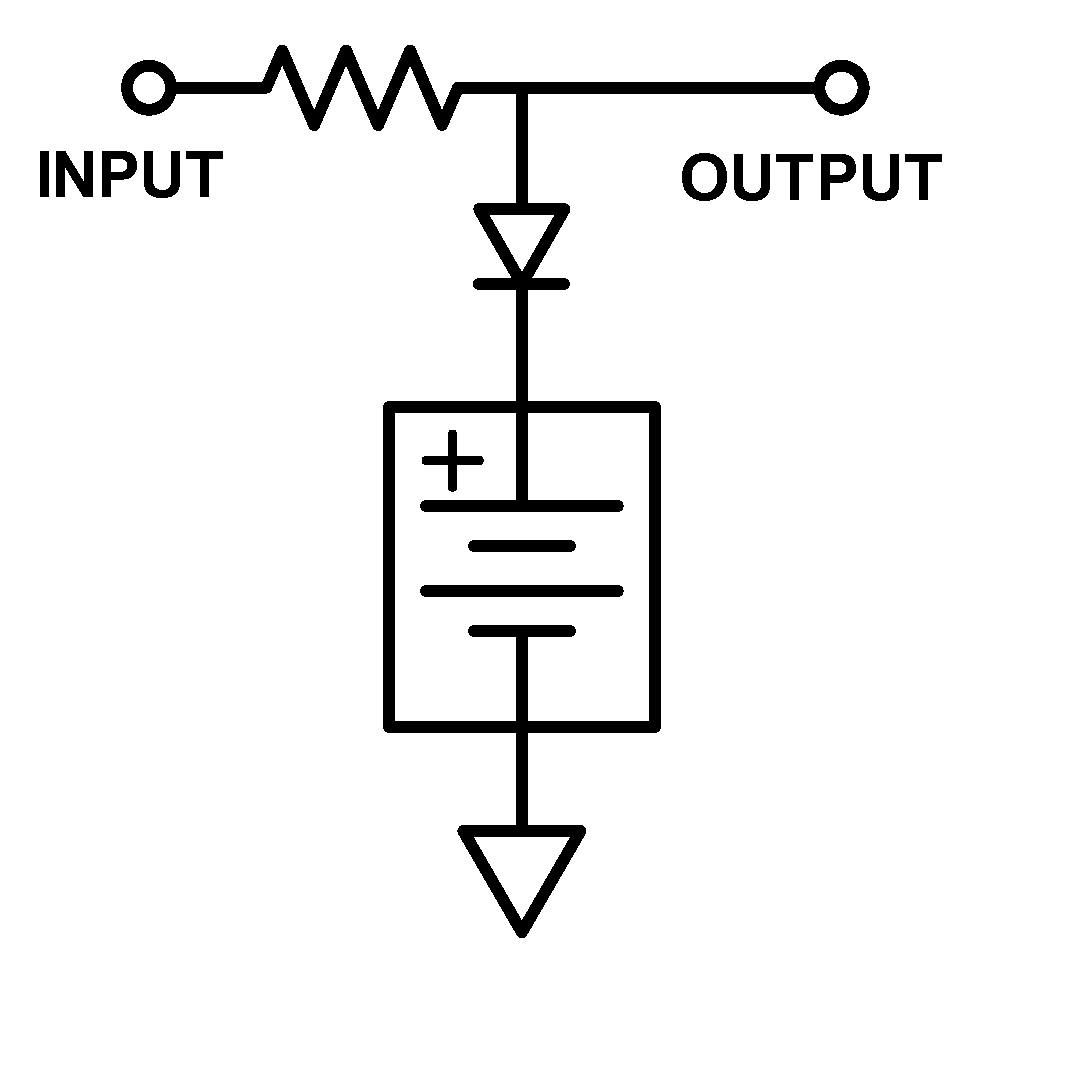
\includegraphics[height=1.2in]{image/Clipping-Circuit.pdf}
        \caption{Clipping circuit cut off higher voltage}
        \label{fig:clippingCircuit}
    \end{figure}
    A clipping circuit can cut off the higher voltage or lowwer voltage. An example is as Figure~\ref{fig:clippingCircuit}. This circuit will cut off higher voltage. If the battery have voltage $\vcc$, than in the positive end of battery the we have voltage $\vcc$. If the diode allow current pass, than voltage on output would be $\vcc + V_d$, where $V_d$ is the voltage drop on diode. We can find the current go through the resistor as 
    \[
    I = \frac{V_\text{in} - \vcc - V_d }{R}
    \]

    On the other hand, if the diode does not allow current pass, that imply the voltage between the diode is smaller than $V_d$. Thus the Output have to smaller than $\vcc + V_d$. Thus, we have following equation:
    \begin{equation}
        V_\text{out} = 
        \begin{cases}
            V_\text{in},    &\text{if } V_\text{in}<\vcc + V_d;\\
            \vcc + V_d,     &\text{if } V_\text{in}\ge\vcc + V_d
        \end{cases} \label{eq:clippingCircuit}
    \end{equation}
    which cut off any voltage higher than $\vcc + V_d$. For example, if one wants to cut off the any voltage higher than 5.6V, we can use a 5V battery.

    \begin{figure}[h]
        \centering
        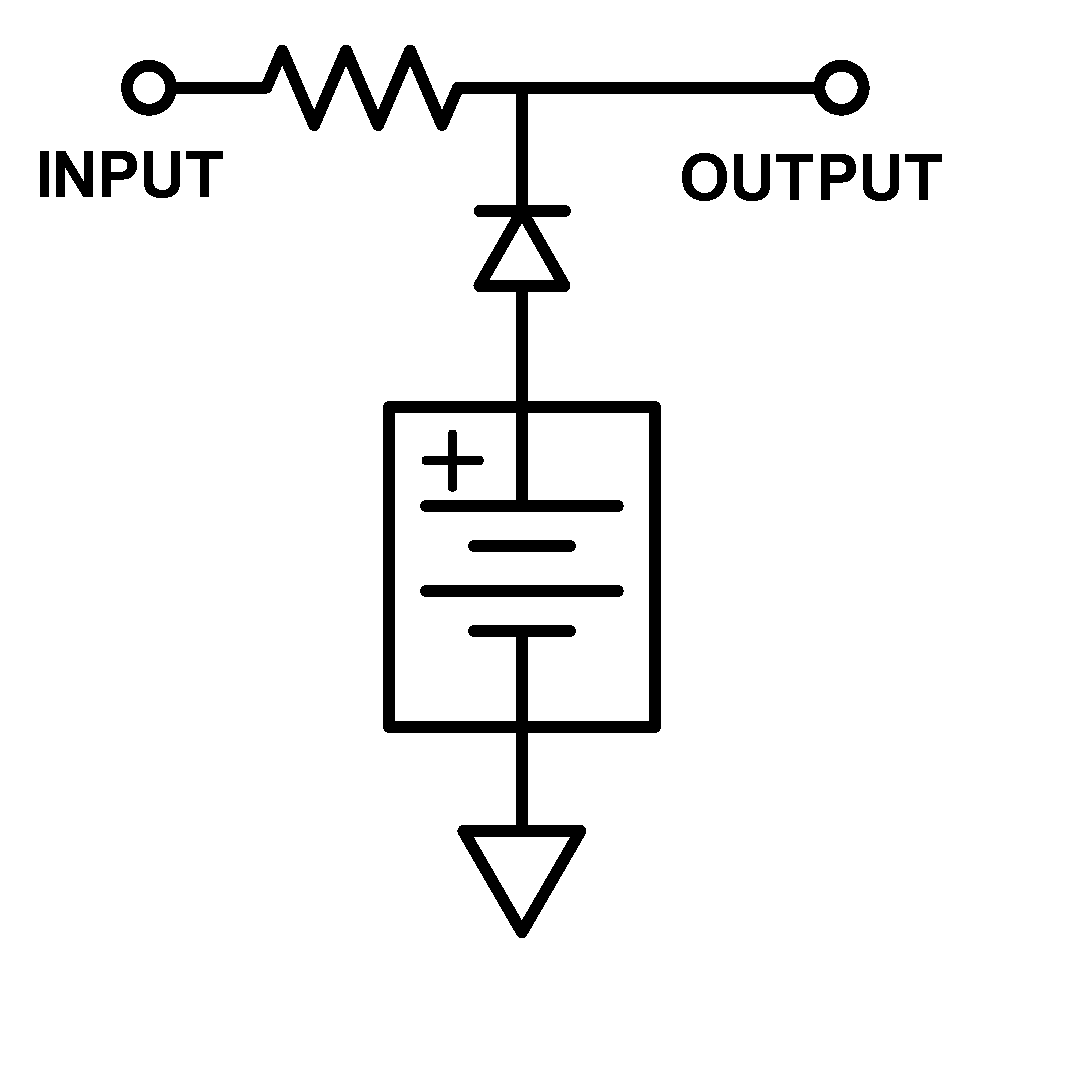
\includegraphics[height=1.2in]{image/Clipping-Circuit-Reverse.pdf}
        \caption{Clipping circuit cut off lowwer voltage}
        \label{fig:clippingCircuitReverse}
    \end{figure}
    In the other hand, we can reverse the diode to form a circuit such as Figure~\ref{fig:clippingCircuitReverse}. This circuit will cut off lowwer voltage. The voltage in the positive end of battery again have to be $\vcc$. This means the voltage in the output is $\vcc - V_d$ when diode can go through current. If the diode cannot go through current, the output voltage have to higher than $\vcc - V_d$. Which suggest
    \begin{equation}
        V_\text{out} = 
        \begin{cases}
            V_\text{in},    &\text{if } V_\text{in}>\vcc - V_d;\\
            \vcc - V_d,     &\text{if } V_\text{in}\le\vcc - V_d
        \end{cases} \label{eq:clippingCircuitReverse}
    \end{equation}

    \begin{figure}[h]
        \centering
        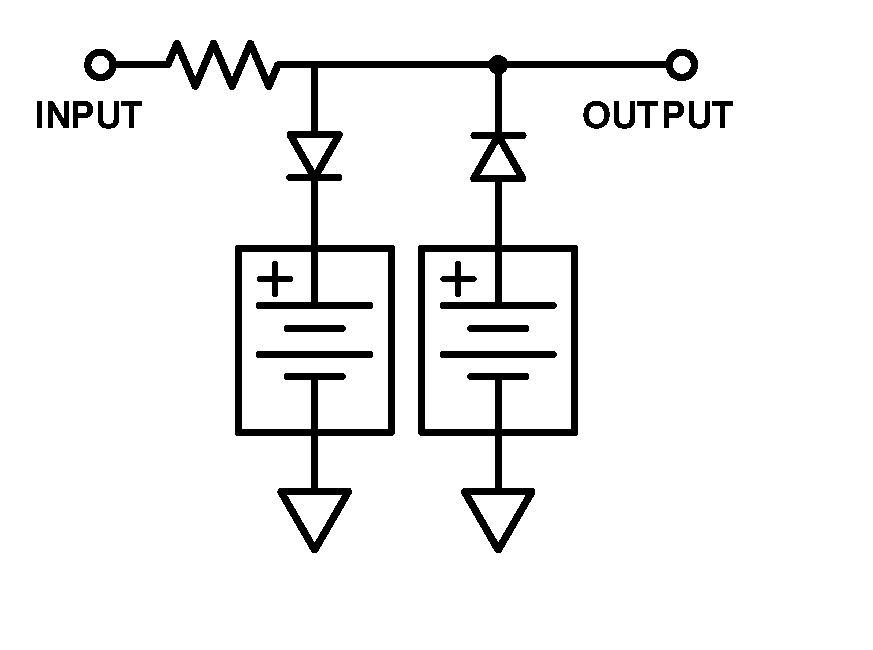
\includegraphics[height=1.2in]{image/Clipping-Circuit-Dual.pdf}
        \caption{Clipping circuit cut off higher and lowwer voltage}
        \label{fig:clippingCircuitDual}
    \end{figure}
    We can also use above two type of clipping circuit to form a circuit such as Figure~\ref{fig:clippingCircuitDual}. Such circuit will cut off higher and lowwer voltage. We can using Equation~\ref{eq:clippingCircuit} and Equation~\ref{eq:clippingCircuitReverse} to find following 
    \begin{equation}
        V_\text{out} = 
        \begin{cases}
            V_\text{cch} + V_d,     &\text{if } V_\text{in}\ge V_\text{cch} + V_d;\\
            V_\text{in},            &\text{if } V_\text{cch} + V_d>V_\text{in}>V_\text{ccl} - V_d;\\
            V_\text{ccl} - V_d,     &\text{if } V_\text{in}\le V_\text{ccl} - V_d
        \end{cases} \label{eq:clippingCircuitDual}
    \end{equation}

    \begin{figure}[h]
        \centering
        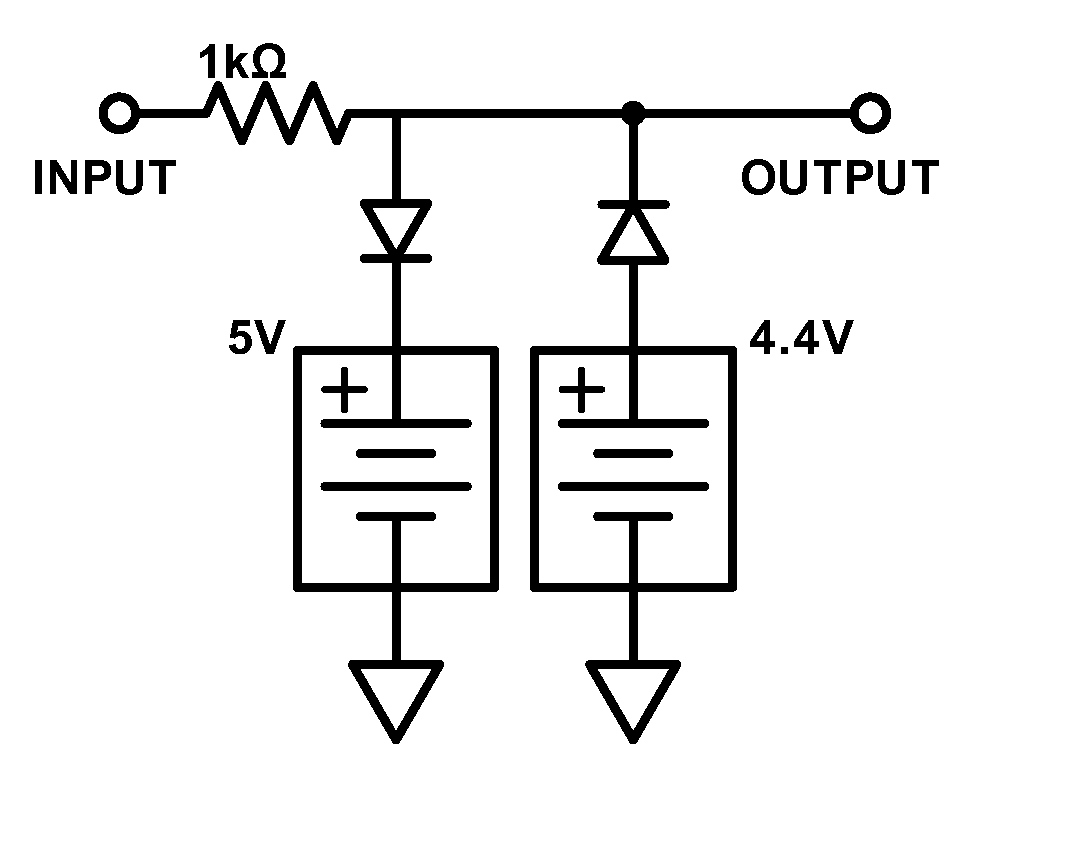
\includegraphics[height=1.2in]{image/Clipping-Circuit-Dual-Lab.pdf}
        \caption{An example of clipping circuit cut off higher and lowwer voltage}
        \label{fig:clippingCircuitDualLab}
    \end{figure}
    For example, if one wans to cut of any voltage higher than 5.6V, and any voltage lowwer than -5V, a 5V battery (for cut off high voltage) and a 4.4V battery (for cut off low voltage). Such as Figure~\ref{fig:clippingCircuitDualLab}.

    \subsection{Full Wave Rectifier}
    \begin{figure}[h]
        \centering
        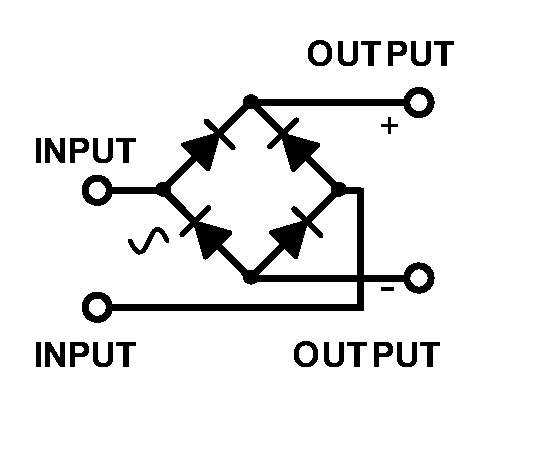
\includegraphics[height=1in]{image/Full-Wave-Rectifier.pdf}
        \caption{Full Wave Rectifier}
        \label{fig:fullWaveRectifier}
    \end{figure}

    A full wave rectifier can transfrom a AC input voltage into a changing positive sign voltage. An example is as Figure~\ref{fig:fullWaveRectifier}. The incomming current can only go from positive to negative as labeled in the output port. When the current go through the full wave rectifier, we can see it will go through a diode. This means the output voltage droped $V_d$.

    \begin{figure}[h]
        \centering
        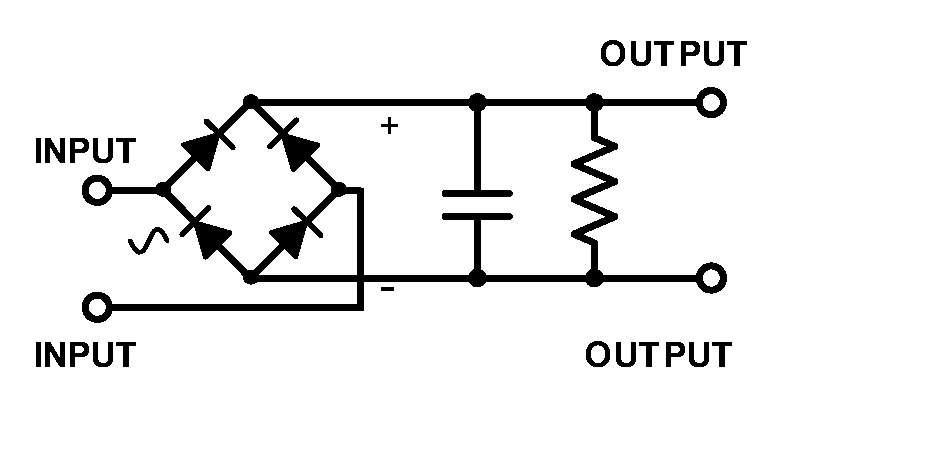
\includegraphics[height=1in]{image/ACDC.pdf}
        \caption{Transfrom AC to DC}
        \label{fig:acdc}
    \end{figure}
    However, such full wave rectifier cannot provide a constent DC output. Thus, we want to smooth the output. A circuit such as Figure~\ref{fig:acdc} can be used to do so. In such circuit, a RC circuit is connect to the output of rectifier. Once the capacitor is charged, it follows the voltage dorp of a RC circuit:
    \begin{equation}
        V(t) = V_0e^{-\frac{t}{RC}} \label{eq:RC}
    \end{equation}
    to drop voltage untill it been charged again. This form a ripple around the peck of output of full wave rectifier. One can use the Equation~\ref{eq:RC} to find the $\Delta V$ of ripple. If the voltage droped slow enough, that is to say, the recharge moment happened almost at the peak, the time that voltage can drop is $\frac{T}{2}$. Thus, using Equation~\ref{eq:RC}, we find:
    \[
    V(\frac{T}{2}) = V_0e^{-\frac{T}{2RC}} \approx V_0 (1 - \frac{T}{2RC})
    \]
    This give us the $\Delta V$ as $V(0) - V(\frac{T}{2})$:
    \begin{equation}
        \Delta V = \frac{V_0 T}{2RC} = \frac{V_0 }{2RCf} \label{eq:fullWaveRectifier}
    \end{equation}

\section{Data and Calculation}
    \subsection{Diode}
    \begin{figure}[H]
        \centering
        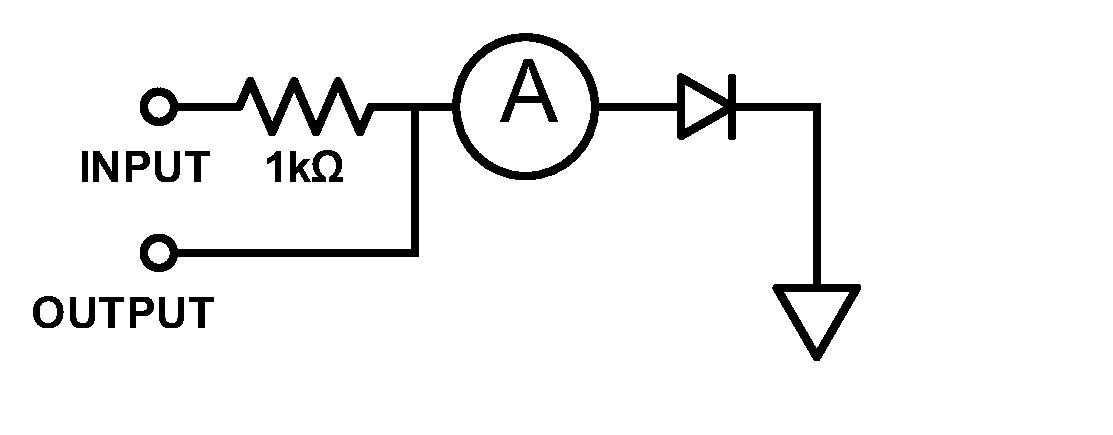
\includegraphics[height=0.7in]{image/Diode-Lab.pdf}
        \caption{Measure the I-V curve of a diode}
        \label{fig:diodeLab}
    \end{figure}
    % \begin{figure}[h]
    %     \centering
    %     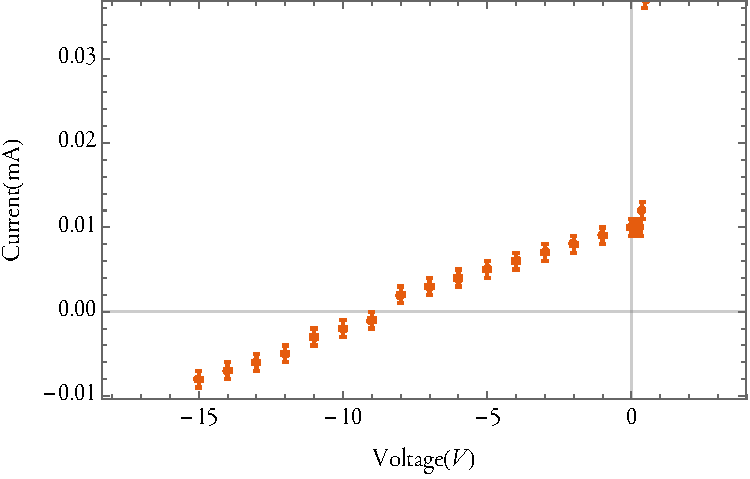
\includegraphics[height=1.8in]{image/Diode-Plot.pdf}
    %     \footnotetext{Some error bar on voltage and current are too small to see}
    %     \caption{I-V curve of a diode}
    %     \label{fig:diodePlot}
    % \end{figure}
    % \begin{figure}[h]
    %     \centering
    %     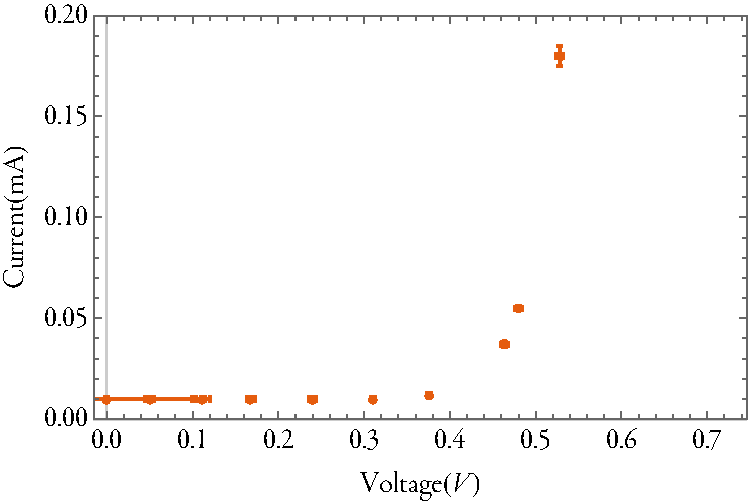
\includegraphics[height=1.8in]{image/Diode-Plot-Close.pdf}
    %     \footnotetext{Some error bar on voltage and current are too small to see}
    %     \caption{A close look of I-V curve of a diode}
    %     \label{fig:diodePlotClose}
    % \end{figure}

    \begin{figure*}[t]
    \centering
    \subcaptionbox{All data point}[.49\linewidth][c]{%
        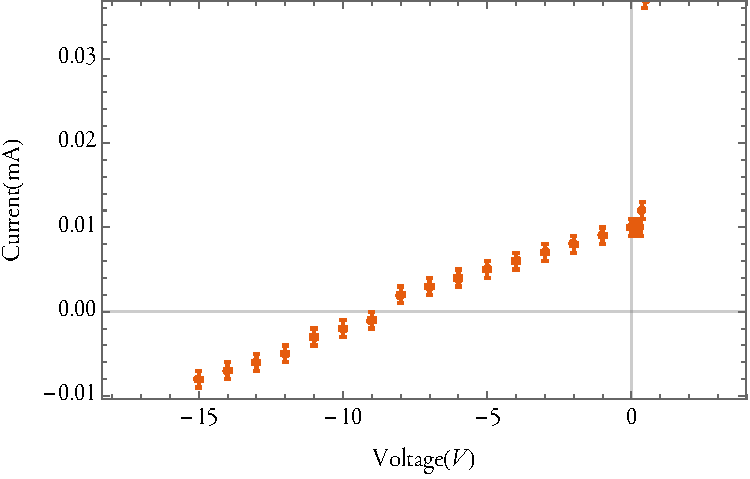
\includegraphics[width=.4\linewidth]{image/Diode-Plot.pdf}}\quad
    \subcaptionbox{A close look}[.49\linewidth][c]{%
        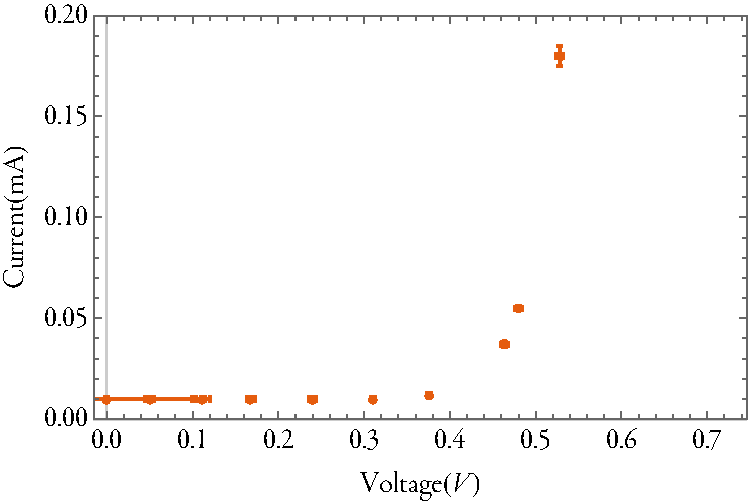
\includegraphics[width=.4\linewidth]{image/Diode-Plot-Close.pdf}}
    \footnotetext{Some error bar on voltage and current are too small to see}
    \footnotetext{Notice the error bar in this range are smaller than others. Some error bar on voltage and current are too small to see}
    \caption{I-V curve of a diode}
    \label{fig:diodePlot}
    \end{figure*}
    To measure the I-V curve of a diode, we use a circuit as Figure~\ref{fig:diodeLab}. Ths resistor is used to protect the circuit. The data we obtained as appendix, error are from the minmum scale of the meter and the changing digit. 

    From the data, one can form a plot as Figure~\ref{fig:diodePlot}a. One may interested on the voltage is larger than 0 smller than $V_d$, such as Figure~\ref{fig:diodePlot}b.

    \subsection{Clipping Circuit}
    \begin{figure}[b]
        \centering
        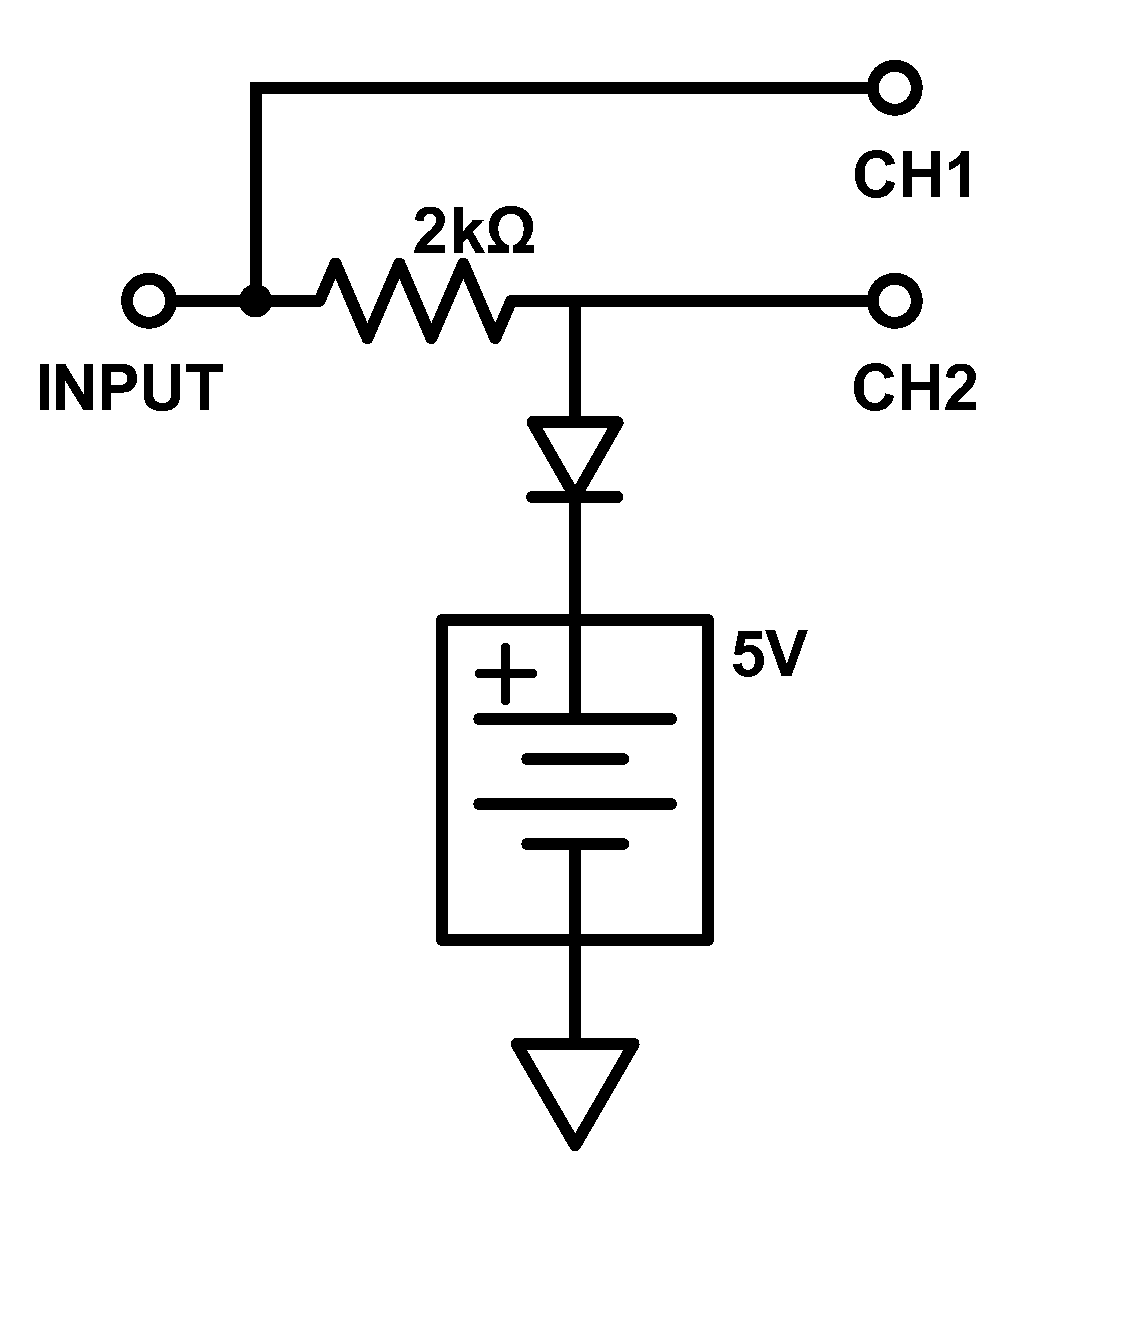
\includegraphics[height=1.2in]{image/Clipping-Circuit-Lab.pdf}
        \caption{Clipping circuit used in lab}
        \label{fig:clippingCircuitLab}
    \end{figure}
    \begin{figure}[b]
        \centering
        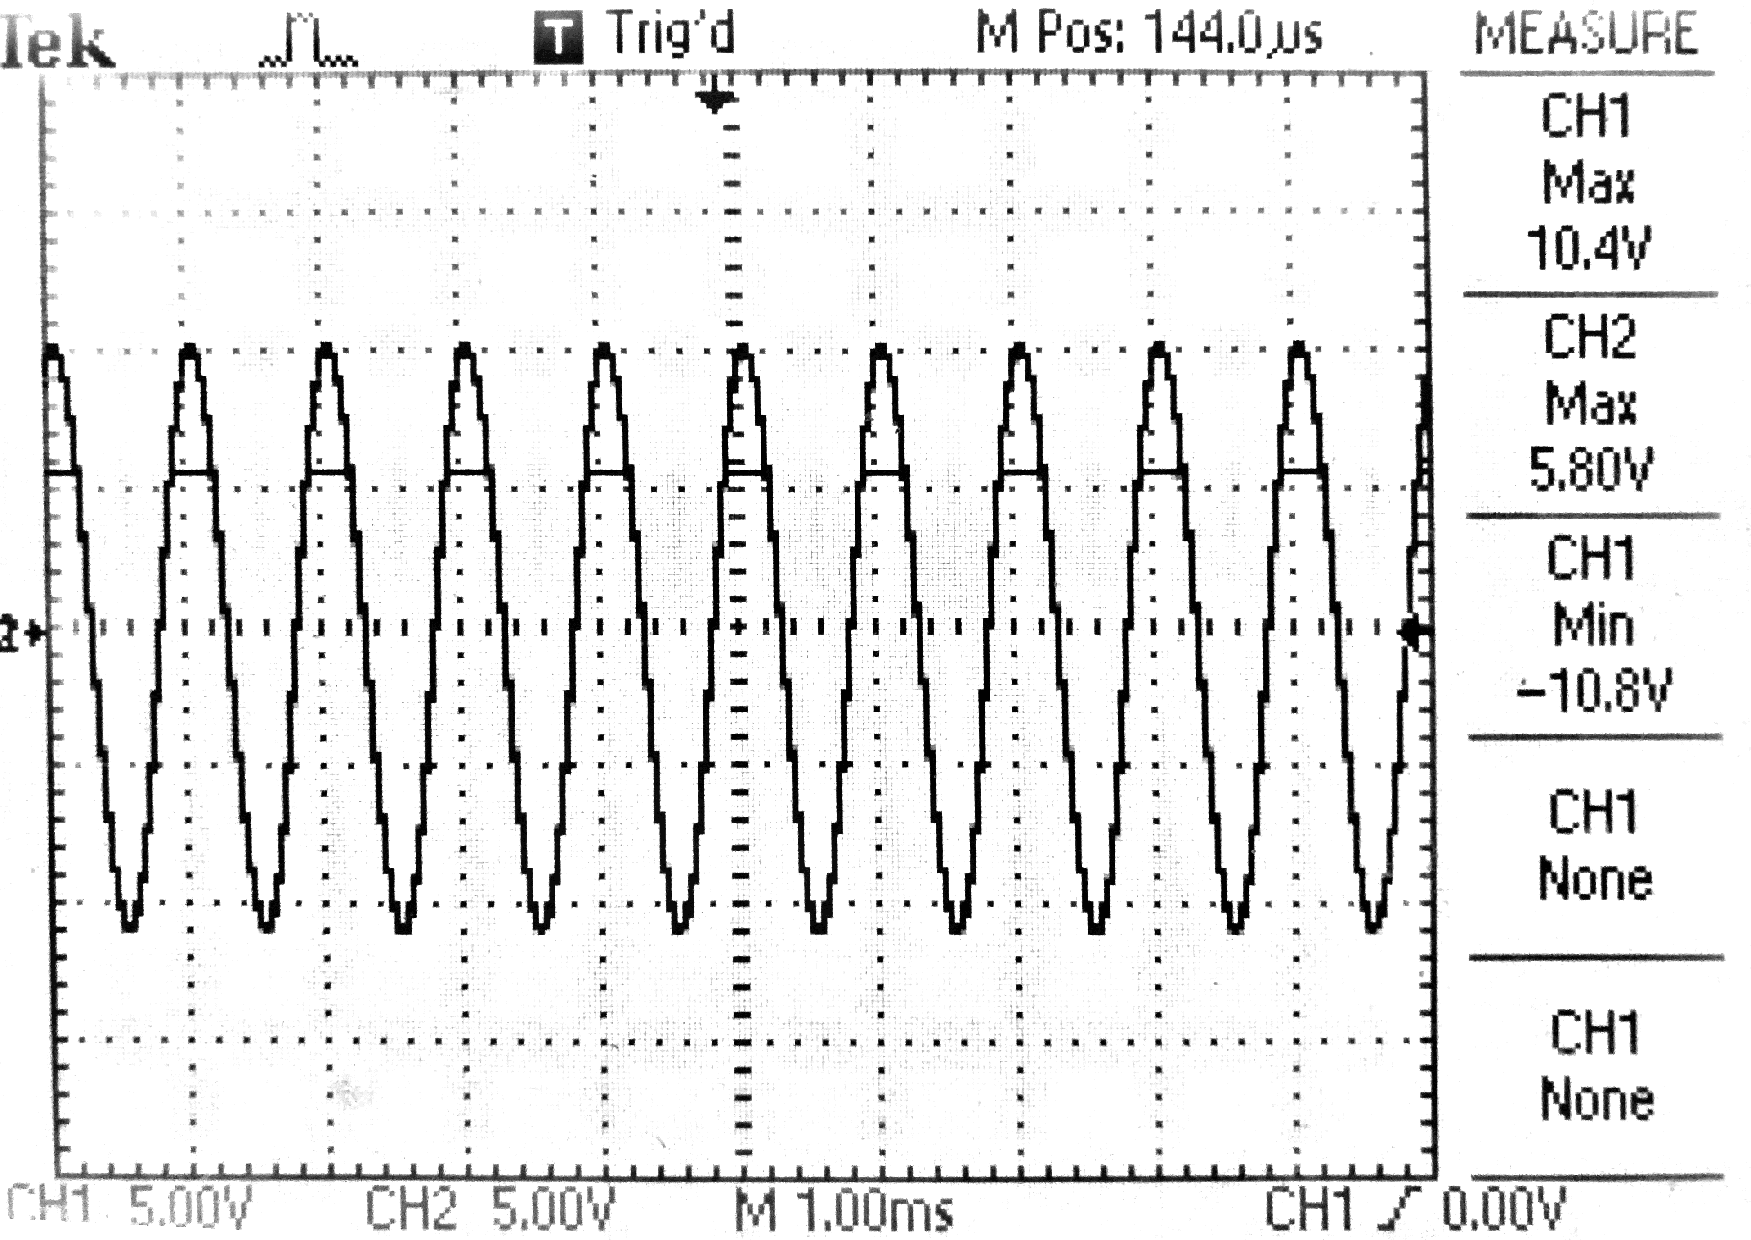
\includegraphics[height=2.2in]{image/Clipping-Scope}
        \caption{Ouput of clipping circuit}
        \label{fig:ClippingScope}
    \end{figure}
    One can make a clipping circuit so that the voltage higher than 5.6V are limited, such as Figure~\ref{fig:clippingCircuitLab}. To do so, one must follow Equation~\ref{eq:clippingCircuit} to find the battery voltage. 
    \begin{align*}
        \vcc &= V_\text{cut} - V_d\\
             &= 5.6V - 0.6V\\
             &= 5V
    \end{align*}
    We assmue the voltage drop on the diode is 0.6V. Therefore, to cut off voltage higher than 5.6V, one have to use a 5V battery. 

    The output of the circuit is as Figure~\ref{fig:ClippingScope}.

    \subsection{Full-Wave Rectifier}
    \begin{figure}[t]
        \centering
        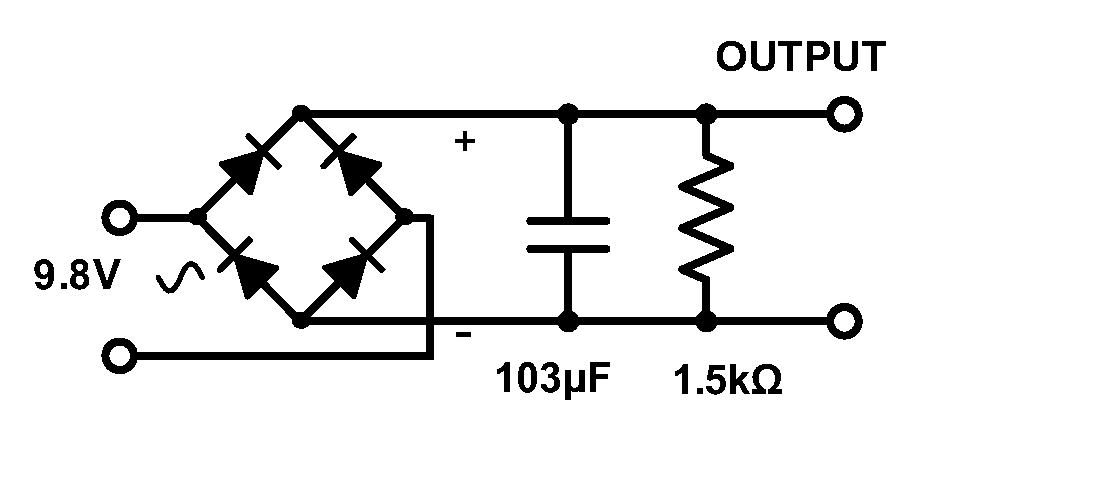
\includegraphics[height=1in]{image/ACDC-Lab.pdf}
        \caption{Full-Wave Rectifier used in lab}
        \label{fig:fullWaveRectifierCircuitLab}
    \end{figure}
    \begin{figure}[t]
        \centering
        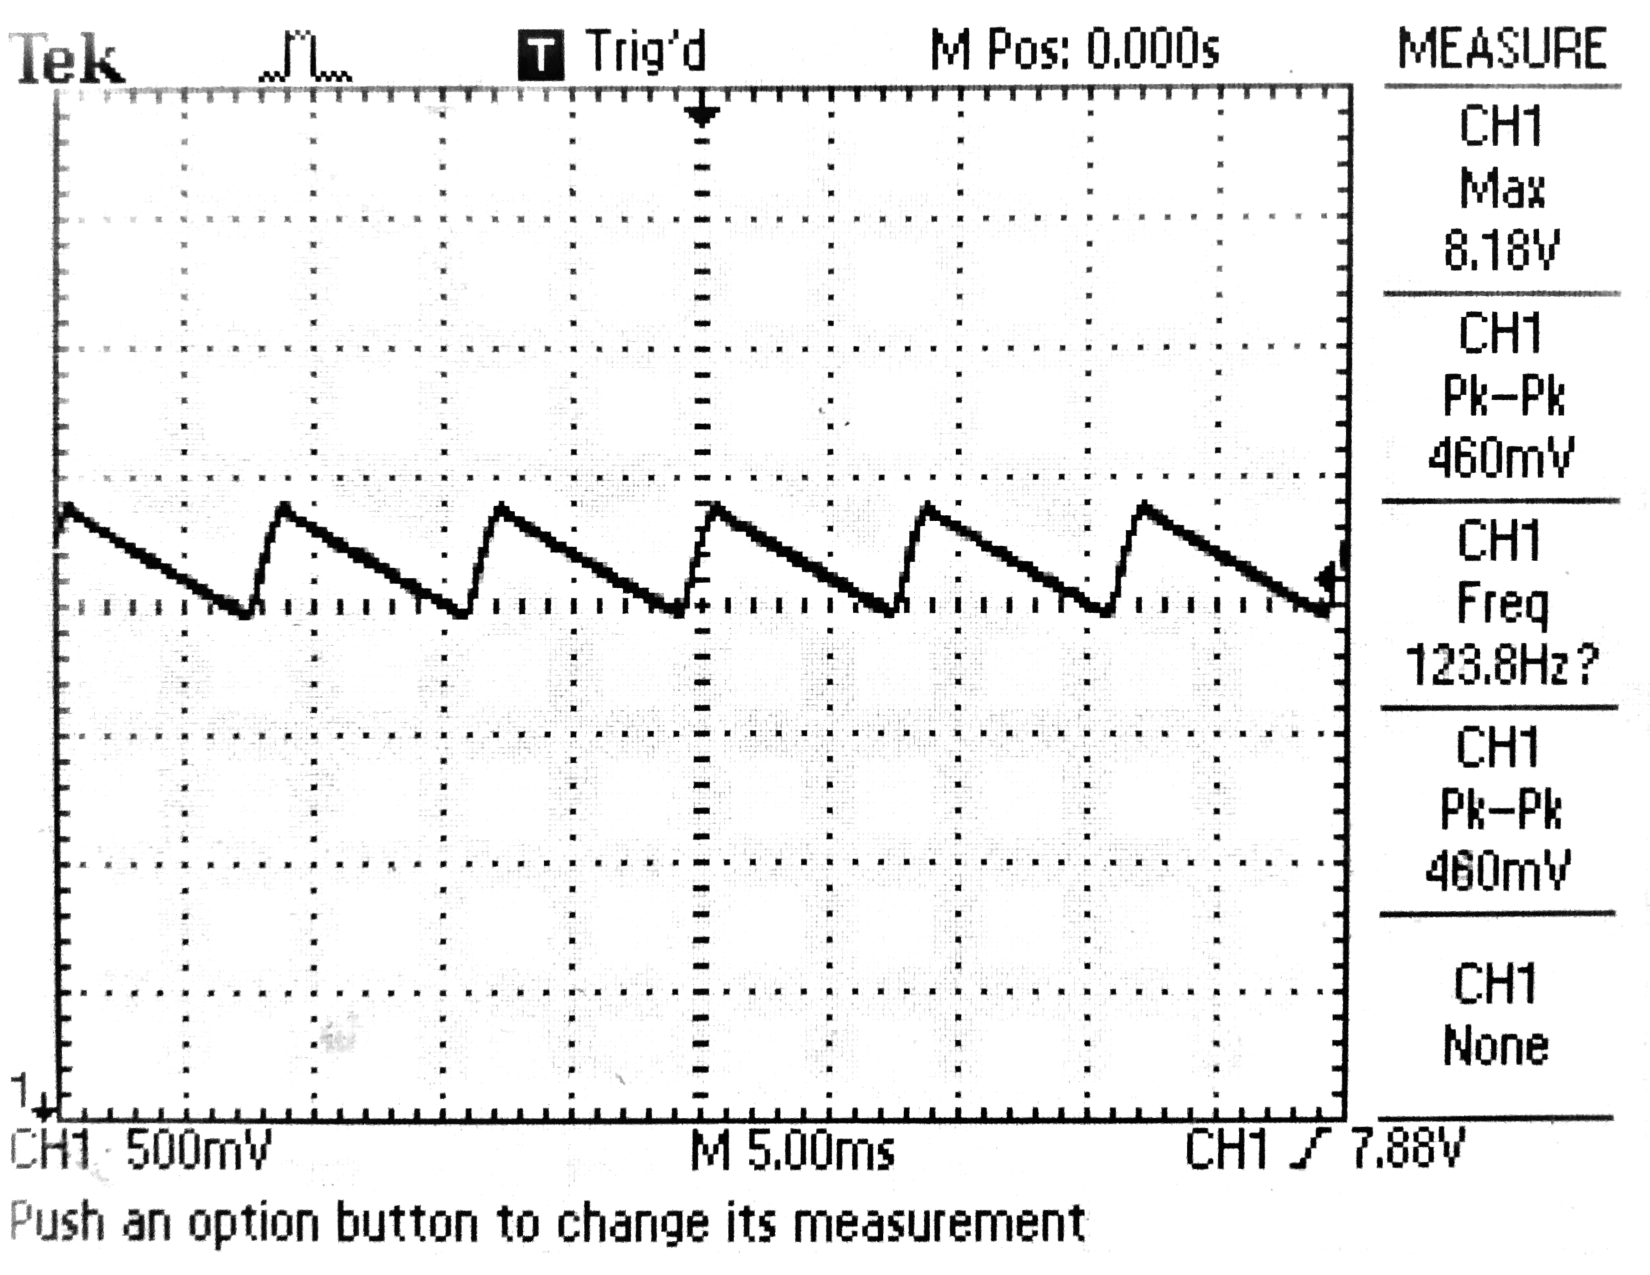
\includegraphics[height=2.2in]{image/Full-Wave-Rectifier-Scope}
        \caption{Ouput of Full-Wave Rectifier}
        \label{fig:fullWaveRectifierScope}
    \end{figure}
    A 9.800(5)V and 60.00(5)Hz AC input voltage are given, to make a full-wave rectifier such that the ripple is around 0.5V, one must use the Equation~\ref{eq:fullWaveRectifier}. 
    \begin{align*}
        \Delta V &=\frac{V_0 }{2RCf} \\
        RC &= \frac{V_0}{2f\Delta V}\\
        &= \frac{9.8V}{2\times 60\text{Hz} \times 0.5V}\\
        &= 0.1633
    \end{align*}
    Thus, the value or RC sould be $0.1633 \Omega F$. In this lab, a 103(1)$\mu$F capacitor and a $1.50(5)$k$\Omega$ resistor are used. 


    Thus, one can form a circuit as Figure~\ref{fig:fullWaveRectifierCircuitLab}. The output of the circuit is as Figure~\ref{fig:fullWaveRectifierScope}. Notice that the output zero voltage line is below the screen.

\section{Analysis}
    \subsection{Diode}
    The result is reasonable. The curve blow up after around 0.6V, which is reasonable for a diode. when voltage is smaller and negtive, the current is small and almost zero. 

    When voltage is negative, at some point, the current is larger than zero, which is not very reasonable. That might due to the background noisy voltage.
    \subsection{Clipping Circuit}
    The output of the circuit is reasonable. It is indeed a clipping circuit that cut off higher voltage. 

    We see the output have maxumum voltage 5.8, which is higher than 5.6V. The diode used in this circuit could have a higher $V_d$. One can use a better diode to achive a better result.
    \subsection{Full-Wave Rectifier}
    The result is reasonable. We obtained a circuit such taht the ripple is around 0.5V. It is almost a DC output.
    
\section{Conclusion}
    The reusult of this lab is reasonable. The only part interesting is when measure the I-V curve of a diode, it gives a positive current when voltage are negative, which might due to the background noisy voltage.

\bibliography{cite}
\bibliographystyle{apsrev4-1}

    % \begin{figure}[h]
    %     \centering
    %     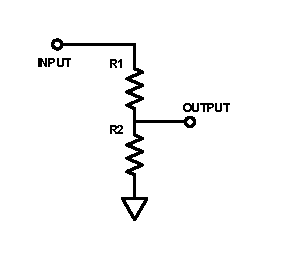
\includegraphics{images/plot2.pdf}
    %     \caption{A voltage divider}
    %     \label{fig:2}
    % \end{figure}

    % \begin{table}[h]
    % \begin{ruledtabular}
    % \begin{tabular}{cccc} 
    % Load[k$\Omega$] &  Output Voltage[V] & $R_\text{th}[\Omega]$ & Theoretical Voltage\\ \hline\hline
    % 50              & 0.680(1)           & 501(1)                & 0.682 \\ \hline
    % 500             & 3.75(1)            & 500(1)                & 3.75 \\ \hline
    % 5000            & 6.80(1)            & 514(1)                & 6.82 \\
    % \end{tabular}
    % \end{ruledtabular}
    % \caption{Load resistor and the output}
    % \label{table:8}
    % \end{table} 

% \begin{center}
%  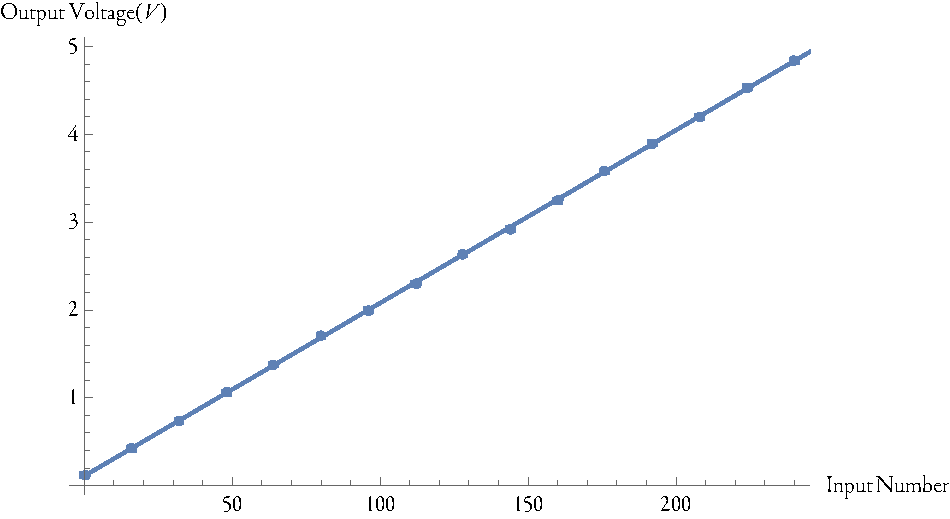
\includegraphics[height=1.8in]{plot.pdf}
% \end{center} 

%\begin{center}
% 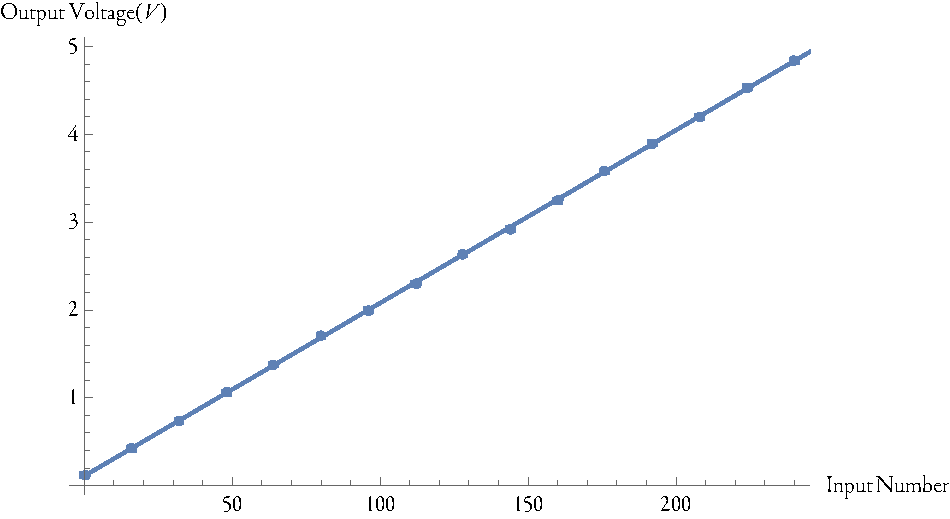
\includegraphics[height=1.3in]{plot.pdf}
%\end{center}

% \blindtext \cite{article-minimal}

% \bibliographystyle{apsrev4-1} % Tell bibtex which bibliography style to use
% \bibliography{xampl} % Tell bibtex which .bib file to use (this one is some example file in TexLive's file tree)

\end{document}